\documentclass[1p]{elsarticle_modified}
%\bibliographystyle{elsarticle-num}

%\usepackage[colorlinks]{hyperref}
%\usepackage{abbrmath_seonhwa} %\Abb, \Ascr, \Acal ,\Abf, \Afrak
\usepackage{amsfonts}
\usepackage{amssymb}
\usepackage{amsmath}
\usepackage{amsthm}
\usepackage{scalefnt}
\usepackage{amsbsy}
\usepackage{kotex}
\usepackage{caption}
\usepackage{subfig}
\usepackage{color}
\usepackage{graphicx}
\usepackage{xcolor} %% white, black, red, green, blue, cyan, magenta, yellow
\usepackage{float}
\usepackage{setspace}
\usepackage{hyperref}

\usepackage{tikz}
\usetikzlibrary{arrows}

\usepackage{multirow}
\usepackage{array} % fixed length table
\usepackage{hhline}

%%%%%%%%%%%%%%%%%%%%%
\makeatletter
\renewcommand*\env@matrix[1][\arraystretch]{%
	\edef\arraystretch{#1}%
	\hskip -\arraycolsep
	\let\@ifnextchar\new@ifnextchar
	\array{*\c@MaxMatrixCols c}}
\makeatother %https://tex.stackexchange.com/questions/14071/how-can-i-increase-the-line-spacing-in-a-matrix
%%%%%%%%%%%%%%%

\usepackage[normalem]{ulem}

\newcommand{\msout}[1]{\ifmmode\text{\sout{\ensuremath{#1}}}\else\sout{#1}\fi}
%SOURCE: \msout is \stkout macro in https://tex.stackexchange.com/questions/20609/strikeout-in-math-mode

\newcommand{\cancel}[1]{
	\ifmmode
	{\color{red}\msout{#1}}
	\else
	{\color{red}\sout{#1}}
	\fi
}

\newcommand{\add}[1]{
	{\color{blue}\uwave{#1}}
}

\newcommand{\replace}[2]{
	\ifmmode
	{\color{red}\msout{#1}}{\color{blue}\uwave{#2}}
	\else
	{\color{red}\sout{#1}}{\color{blue}\uwave{#2}}
	\fi
}

\newcommand{\Sol}{\mathcal{S}} %segment
\newcommand{\D}{D} %diagram
\newcommand{\A}{\mathcal{A}} %arc


%%%%%%%%%%%%%%%%%%%%%%%%%%%%%5 test

\def\sl{\operatorname{\textup{SL}}(2,\Cbb)}
\def\psl{\operatorname{\textup{PSL}}(2,\Cbb)}
\def\quan{\mkern 1mu \triangleright \mkern 1mu}

\theoremstyle{definition}
\newtheorem{thm}{Theorem}[section]
\newtheorem{prop}[thm]{Proposition}
\newtheorem{lem}[thm]{Lemma}
\newtheorem{ques}[thm]{Question}
\newtheorem{cor}[thm]{Corollary}
\newtheorem{defn}[thm]{Definition}
\newtheorem{exam}[thm]{Example}
\newtheorem{rmk}[thm]{Remark}
\newtheorem{alg}[thm]{Algorithm}

\newcommand{\I}{\sqrt{-1}}
\begin{document}

%\begin{frontmatter}
%
%\title{Boundary parabolic representations of knots up to 8 crossings}
%
%%% Group authors per affiliation:
%\author{Yunhi Cho} 
%\address{Department of Mathematics, University of Seoul, Seoul, Korea}
%\ead{yhcho@uos.ac.kr}
%
%
%\author{Seonhwa Kim} %\fnref{s_kim}}
%\address{Center for Geometry and Physics, Institute for Basic Science, Pohang, 37673, Korea}
%\ead{ryeona17@ibs.re.kr}
%
%\author{Hyuk Kim}
%\address{Department of Mathematical Sciences, Seoul National University, Seoul 08826, Korea}
%\ead{hyukkim@snu.ac.kr}
%
%\author{Seokbeom Yoon}
%\address{Department of Mathematical Sciences, Seoul National University, Seoul, 08826,  Korea}
%\ead{sbyoon15@snu.ac.kr}
%
%\begin{abstract}
%We find all boundary parabolic representation of knots up to 8 crossings.
%
%\end{abstract}
%\begin{keyword}
%    \MSC[2010] 57M25 
%\end{keyword}
%
%\end{frontmatter}

%\linenumbers
%\tableofcontents
%
\newcommand\colored[1]{\textcolor{white}{\rule[-0.35ex]{0.8em}{1.4ex}}\kern-0.8em\color{red} #1}%
%\newcommand\colored[1]{\textcolor{white}{ #1}\kern-2.17ex	\textcolor{white}{ #1}\kern-1.81ex	\textcolor{white}{ #1}\kern-2.15ex\color{red}#1	}

{\Large $\underline{12a_{1238}~(K12a_{1238})}$}

\setlength{\tabcolsep}{10pt}
\renewcommand{\arraystretch}{1.6}
\vspace{1cm}\begin{tabular}{m{100pt}>{\centering\arraybackslash}m{274pt}}
\multirow{5}{120pt}{
	\centering
	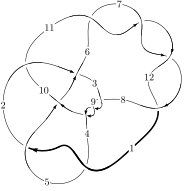
\includegraphics[width=112pt]{../../../GIT/diagram.site/Diagrams/png/2039_12a_1238.png}\\
\ \ \ A knot diagram\footnotemark}&
\allowdisplaybreaks
\textbf{Linearized knot diagam} \\
\cline{2-2}
 &
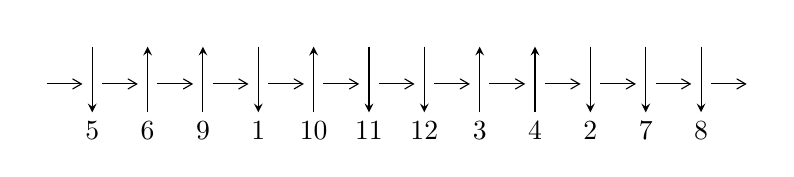
\begin{tikzpicture}[x=20pt, y=17pt]
	% nodes
	\node (C0) at (0, 0) {};
	\node (C1) at (1, 0) {};
	\node (C1U) at (1, +1) {};
	\node (C1D) at (1, -1) {5};

	\node (C2) at (2, 0) {};
	\node (C2U) at (2, +1) {};
	\node (C2D) at (2, -1) {6};

	\node (C3) at (3, 0) {};
	\node (C3U) at (3, +1) {};
	\node (C3D) at (3, -1) {9};

	\node (C4) at (4, 0) {};
	\node (C4U) at (4, +1) {};
	\node (C4D) at (4, -1) {1};

	\node (C5) at (5, 0) {};
	\node (C5U) at (5, +1) {};
	\node (C5D) at (5, -1) {10};

	\node (C6) at (6, 0) {};
	\node (C6U) at (6, +1) {};
	\node (C6D) at (6, -1) {11};

	\node (C7) at (7, 0) {};
	\node (C7U) at (7, +1) {};
	\node (C7D) at (7, -1) {12};

	\node (C8) at (8, 0) {};
	\node (C8U) at (8, +1) {};
	\node (C8D) at (8, -1) {3};

	\node (C9) at (9, 0) {};
	\node (C9U) at (9, +1) {};
	\node (C9D) at (9, -1) {4};

	\node (C10) at (10, 0) {};
	\node (C10U) at (10, +1) {};
	\node (C10D) at (10, -1) {2};

	\node (C11) at (11, 0) {};
	\node (C11U) at (11, +1) {};
	\node (C11D) at (11, -1) {7};

	\node (C12) at (12, 0) {};
	\node (C12U) at (12, +1) {};
	\node (C12D) at (12, -1) {8};
	\node (C13) at (13, 0) {};

	% arrows
	\draw[->,>={angle 60}]
	(C0) edge (C1) (C1) edge (C2) (C2) edge (C3) (C3) edge (C4) (C4) edge (C5) (C5) edge (C6) (C6) edge (C7) (C7) edge (C8) (C8) edge (C9) (C9) edge (C10) (C10) edge (C11) (C11) edge (C12) (C12) edge (C13) ;	\draw[->,>=stealth]
	(C1U) edge (C1D) (C2D) edge (C2U) (C3D) edge (C3U) (C4U) edge (C4D) (C5D) edge (C5U) (C6U) edge (C6D) (C7U) edge (C7D) (C8D) edge (C8U) (C9D) edge (C9U) (C10U) edge (C10D) (C11U) edge (C11D) (C12U) edge (C12D) ;
	\end{tikzpicture} \\
\hhline{~~} \\& 
\textbf{Solving Sequence} \\ \cline{2-2} 
 &
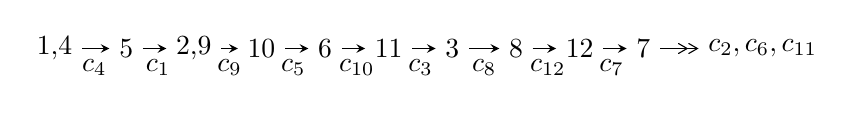
\begin{tikzpicture}[x=23pt, y=7pt]
	% node
	\node (A0) at (-1/8, 0) {1,4};
	\node (A1) at (1, 0) {5};
	\node (A2) at (33/16, 0) {2,9};
	\node (A3) at (25/8, 0) {10};
	\node (A4) at (33/8, 0) {6};
	\node (A5) at (41/8, 0) {11};
	\node (A6) at (49/8, 0) {3};
	\node (A7) at (57/8, 0) {8};
	\node (A8) at (65/8, 0) {12};
	\node (A9) at (73/8, 0) {7};
	\node (C1) at (1/2, -1) {$c_{4}$};
	\node (C2) at (3/2, -1) {$c_{1}$};
	\node (C3) at (21/8, -1) {$c_{9}$};
	\node (C4) at (29/8, -1) {$c_{5}$};
	\node (C5) at (37/8, -1) {$c_{10}$};
	\node (C6) at (45/8, -1) {$c_{3}$};
	\node (C7) at (53/8, -1) {$c_{8}$};
	\node (C8) at (61/8, -1) {$c_{12}$};
	\node (C9) at (69/8, -1) {$c_{7}$};
	\node (A10) at (11, 0) {$c_{2},c_{6},c_{11}$};

	% edge
	\draw[->,>=stealth]	
	(A0) edge (A1) (A1) edge (A2) (A2) edge (A3) (A3) edge (A4) (A4) edge (A5) (A5) edge (A6) (A6) edge (A7) (A7) edge (A8) (A8) edge (A9) ;
	\draw[->>,>={angle 60}]	
	(A9) edge (A10);
\end{tikzpicture} \\ 

\end{tabular} \\

\footnotetext{
The image of knot diagram is generated by the software ``\textbf{Draw programme}" developed by Andrew Bartholomew(\url{http://www.layer8.co.uk/maths/draw/index.htm\#Running-draw}), where we modified some parts for our purpose(\url{https://github.com/CATsTAILs/LinksPainter}).
}\phantom \\ \newline 
\centering \textbf{Ideals for irreducible components\footnotemark of $X_{\text{par}}$} 
 
\begin{align*}
I^u_{1}&=\langle 
1.62330\times10^{233} u^{81}-1.12307\times10^{233} u^{80}+\cdots+7.45191\times10^{232} b+8.93587\times10^{234},\\
\phantom{I^u_{1}}&\phantom{= \langle  }-1.56282\times10^{234} u^{81}-3.71971\times10^{233} u^{80}+\cdots+3.72595\times10^{233} a-2.44109\times10^{236},\\
\phantom{I^u_{1}}&\phantom{= \langle  }u^{82}-29 u^{80}+\cdots+580 u+25\rangle \\
I^u_{2}&=\langle 
-57 u^{16}+139 u^{15}+\cdots+b+105,\;18 u^{16}-43 u^{15}+\cdots+a-24,\;u^{17}-3 u^{16}+\cdots-3 u+1\rangle \\
\\
\end{align*}
\raggedright * 2 irreducible components of $\dim_{\mathbb{C}}=0$, with total 99 representations.\\
\footnotetext{All coefficients of polynomials are rational numbers. But the coefficients are sometimes approximated in decimal forms when there is not enough margin.}
\newpage
\renewcommand{\arraystretch}{1}
\centering \section*{I. $I^u_{1}= \langle 1.62\times10^{233} u^{81}-1.12\times10^{233} u^{80}+\cdots+7.45\times10^{232} b+8.94\times10^{234},\;-1.56\times10^{234} u^{81}-3.72\times10^{233} u^{80}+\cdots+3.73\times10^{233} a-2.44\times10^{236},\;u^{82}-29 u^{80}+\cdots+580 u+25 \rangle$}
\flushleft \textbf{(i) Arc colorings}\\
\begin{tabular}{m{7pt} m{180pt} m{7pt} m{180pt} }
\flushright $a_{1}=$&$\begin{pmatrix}0\\u\end{pmatrix}$ \\
\flushright $a_{4}=$&$\begin{pmatrix}1\\0\end{pmatrix}$ \\
\flushright $a_{5}=$&$\begin{pmatrix}1\\u^2\end{pmatrix}$ \\
\flushright $a_{2}=$&$\begin{pmatrix}- u\\- u^3+u\end{pmatrix}$ \\
\flushright $a_{9}=$&$\begin{pmatrix}4.19443 u^{81}+0.998323 u^{80}+\cdots+12103.0 u+655.158\\-2.17837 u^{81}+1.50709 u^{80}+\cdots-2279.85 u-119.914\end{pmatrix}$ \\
\flushright $a_{10}=$&$\begin{pmatrix}2.01606 u^{81}+2.50541 u^{80}+\cdots+9823.13 u+535.245\\-2.17837 u^{81}+1.50709 u^{80}+\cdots-2279.85 u-119.914\end{pmatrix}$ \\
\flushright $a_{6}=$&$\begin{pmatrix}4.65242 u^{81}-1.59030 u^{80}+\cdots+8732.87 u+474.826\\-2.43795 u^{81}+1.31148 u^{80}+\cdots-3819.62 u-208.334\end{pmatrix}$ \\
\flushright $a_{11}=$&$\begin{pmatrix}3.51386 u^{81}+1.04832 u^{80}+\cdots+10330.4 u+553.673\\-2.43681 u^{81}+1.96106 u^{80}+\cdots-1979.41 u-101.915\end{pmatrix}$ \\
\flushright $a_{3}=$&$\begin{pmatrix}-7.59176 u^{81}+2.77225 u^{80}+\cdots-13921.6 u-746.885\\0.100451 u^{81}+0.634586 u^{80}+\cdots+2030.94 u+123.163\end{pmatrix}$ \\
\flushright $a_{8}=$&$\begin{pmatrix}4.09643 u^{81}-2.86268 u^{80}+\cdots+2668.54 u+89.1960\\3.37277 u^{81}-1.62221 u^{80}+\cdots+4955.44 u+259.192\end{pmatrix}$ \\
\flushright $a_{12}=$&$\begin{pmatrix}2.14385 u^{81}-0.151279 u^{80}+\cdots+4824.36 u+223.253\\2.86534 u^{81}-0.999373 u^{80}+\cdots+5564.66 u+300.621\end{pmatrix}$ \\
\flushright $a_{7}=$&$\begin{pmatrix}-4.86395 u^{81}+0.711191 u^{80}+\cdots-10254.4 u-525.349\\-2.54931 u^{81}+1.00523 u^{80}+\cdots-4203.94 u-218.636\end{pmatrix}$\\&\end{tabular}
\flushleft \textbf{(ii) Obstruction class $= -1$}\\~\\
\flushleft \textbf{(iii) Cusp Shapes $= 2.46764 u^{81}+2.98675 u^{80}+\cdots+13265.8 u+747.283$}\\~\\
\newpage\renewcommand{\arraystretch}{1}
\flushleft \textbf{(iv) u-Polynomials at the component}\newline \\
\begin{tabular}{m{50pt}|m{274pt}}
Crossings & \hspace{64pt}u-Polynomials at each crossing \\
\hline $$\begin{aligned}c_{1},c_{4}\end{aligned}$$&$\begin{aligned}
&u^{82}-29 u^{80}+\cdots+580 u+25
\end{aligned}$\\
\hline $$\begin{aligned}c_{2}\end{aligned}$$&$\begin{aligned}
&u^{82}-5 u^{81}+\cdots+2079 u+931
\end{aligned}$\\
\hline $$\begin{aligned}c_{3},c_{8},c_{9}\end{aligned}$$&$\begin{aligned}
&u^{82}- u^{81}+\cdots+181 u+173
\end{aligned}$\\
\hline $$\begin{aligned}c_{5}\end{aligned}$$&$\begin{aligned}
&u^{82}+2 u^{81}+\cdots+17 u-1
\end{aligned}$\\
\hline $$\begin{aligned}c_{6},c_{7},c_{11}\\c_{12}\end{aligned}$$&$\begin{aligned}
&u^{82}- u^{81}+\cdots-79 u-7
\end{aligned}$\\
\hline $$\begin{aligned}c_{10}\end{aligned}$$&$\begin{aligned}
&u^{82}+2 u^{81}+\cdots-3884 u+1867
\end{aligned}$\\
\hline
\end{tabular}\\~\\
\newpage\renewcommand{\arraystretch}{1}
\flushleft \textbf{(v) Riley Polynomials at the component}\newline \\
\begin{tabular}{m{50pt}|m{274pt}}
Crossings & \hspace{64pt}Riley Polynomials at each crossing \\
\hline $$\begin{aligned}c_{1},c_{4}\end{aligned}$$&$\begin{aligned}
&y^{82}-58 y^{81}+\cdots-62350 y+625
\end{aligned}$\\
\hline $$\begin{aligned}c_{2}\end{aligned}$$&$\begin{aligned}
&y^{82}+15 y^{81}+\cdots+9331805 y+866761
\end{aligned}$\\
\hline $$\begin{aligned}c_{3},c_{8},c_{9}\end{aligned}$$&$\begin{aligned}
&y^{82}-77 y^{81}+\cdots+235043 y+29929
\end{aligned}$\\
\hline $$\begin{aligned}c_{5}\end{aligned}$$&$\begin{aligned}
&y^{82}+64 y^{80}+\cdots-209 y+1
\end{aligned}$\\
\hline $$\begin{aligned}c_{6},c_{7},c_{11}\\c_{12}\end{aligned}$$&$\begin{aligned}
&y^{82}-101 y^{81}+\cdots-2405 y+49
\end{aligned}$\\
\hline $$\begin{aligned}c_{10}\end{aligned}$$&$\begin{aligned}
&y^{82}-34 y^{81}+\cdots-204854804 y+3485689
\end{aligned}$\\
\hline
\end{tabular}\\~\\
\newpage\flushleft \textbf{(vi) Complex Volumes and Cusp Shapes}
$$\begin{array}{c|c|c}  
\text{Solutions to }I^u_{1}& \I (\text{vol} + \sqrt{-1}CS) & \text{Cusp shape}\\
 \hline 
\begin{aligned}
u &= -0.934521 + 0.347459 I \\
a &= \phantom{-}0.256869 - 0.427602 I \\
b &= \phantom{-}0.366312 - 0.532440 I\end{aligned}
 & -1.56095 + 1.32976 I & \phantom{-0.000000 } 0 \\ \hline\begin{aligned}
u &= -0.934521 - 0.347459 I \\
a &= \phantom{-}0.256869 + 0.427602 I \\
b &= \phantom{-}0.366312 + 0.532440 I\end{aligned}
 & -1.56095 - 1.32976 I & \phantom{-0.000000 } 0 \\ \hline\begin{aligned}
u &= -0.985856 + 0.133508 I \\
a &= \phantom{-}1.42926 - 1.69263 I \\
b &= -1.338240 - 0.226304 I\end{aligned}
 & -0.18186 + 2.94088 I & \phantom{-0.000000 } 0 \\ \hline\begin{aligned}
u &= -0.985856 - 0.133508 I \\
a &= \phantom{-}1.42926 + 1.69263 I \\
b &= -1.338240 + 0.226304 I\end{aligned}
 & -0.18186 - 2.94088 I & \phantom{-0.000000 } 0 \\ \hline\begin{aligned}
u &= \phantom{-}0.680966 + 0.774466 I \\
a &= -1.285520 - 0.554886 I \\
b &= \phantom{-}1.343090 + 0.338900 I\end{aligned}
 & -3.26211 + 2.41526 I & \phantom{-0.000000 } 0 \\ \hline\begin{aligned}
u &= \phantom{-}0.680966 - 0.774466 I \\
a &= -1.285520 + 0.554886 I \\
b &= \phantom{-}1.343090 - 0.338900 I\end{aligned}
 & -3.26211 - 2.41526 I & \phantom{-0.000000 } 0 \\ \hline\begin{aligned}
u &= \phantom{-}0.943857\phantom{ +0.000000I} \\
a &= \phantom{-}1.46985\phantom{ +0.000000I} \\
b &= -1.84151\phantom{ +0.000000I}\end{aligned}
 & -0.856208\phantom{ +0.000000I} & \phantom{-0.000000 } 0 \\ \hline\begin{aligned}
u &= \phantom{-}0.000750 + 0.932894 I \\
a &= -1.87427 - 0.30470 I \\
b &= \phantom{-}1.45322 - 0.06591 I\end{aligned}
 & \phantom{-}7.14647 - 2.26483 I & \phantom{-0.000000 } 0 \\ \hline\begin{aligned}
u &= \phantom{-}0.000750 - 0.932894 I \\
a &= -1.87427 + 0.30470 I \\
b &= \phantom{-}1.45322 + 0.06591 I\end{aligned}
 & \phantom{-}7.14647 + 2.26483 I & \phantom{-0.000000 } 0 \\ \hline\begin{aligned}
u &= -1.066400 + 0.200953 I \\
a &= -1.82922 + 1.16741 I \\
b &= \phantom{-}1.46675 + 0.30221 I\end{aligned}
 & -7.87907 + 6.39586 I & \phantom{-0.000000 } 0\\
 \hline 
 \end{array}$$\newpage$$\begin{array}{c|c|c}  
\text{Solutions to }I^u_{1}& \I (\text{vol} + \sqrt{-1}CS) & \text{Cusp shape}\\
 \hline 
\begin{aligned}
u &= -1.066400 - 0.200953 I \\
a &= -1.82922 - 1.16741 I \\
b &= \phantom{-}1.46675 - 0.30221 I\end{aligned}
 & -7.87907 - 6.39586 I & \phantom{-0.000000 } 0 \\ \hline\begin{aligned}
u &= -0.738427 + 0.486038 I \\
a &= -0.819329 + 0.132184 I \\
b &= -0.131483 + 0.984194 I\end{aligned}
 & -7.99328 + 2.08374 I & \phantom{-0.000000 } 0 \\ \hline\begin{aligned}
u &= -0.738427 - 0.486038 I \\
a &= -0.819329 - 0.132184 I \\
b &= -0.131483 - 0.984194 I\end{aligned}
 & -7.99328 - 2.08374 I & \phantom{-0.000000 } 0 \\ \hline\begin{aligned}
u &= \phantom{-}0.937847 + 0.605715 I \\
a &= \phantom{-}1.39663 + 1.28141 I \\
b &= -1.35817 + 0.50981 I\end{aligned}
 & -4.06787 - 7.61264 I & \phantom{-0.000000 } 0 \\ \hline\begin{aligned}
u &= \phantom{-}0.937847 - 0.605715 I \\
a &= \phantom{-}1.39663 - 1.28141 I \\
b &= -1.35817 - 0.50981 I\end{aligned}
 & -4.06787 + 7.61264 I & \phantom{-0.000000 } 0 \\ \hline\begin{aligned}
u &= -0.164401 + 1.104770 I \\
a &= -0.068114 + 0.588364 I \\
b &= -0.219137 - 0.621589 I\end{aligned}
 & -8.99433 + 5.16744 I & \phantom{-0.000000 } 0 \\ \hline\begin{aligned}
u &= -0.164401 - 1.104770 I \\
a &= -0.068114 - 0.588364 I \\
b &= -0.219137 + 0.621589 I\end{aligned}
 & -8.99433 - 5.16744 I & \phantom{-0.000000 } 0 \\ \hline\begin{aligned}
u &= -1.086900 + 0.269679 I \\
a &= \phantom{-}0.334063 + 0.325688 I \\
b &= -0.863302 + 0.735990 I\end{aligned}
 & -3.51083 + 2.83032 I & \phantom{-0.000000 } 0 \\ \hline\begin{aligned}
u &= -1.086900 - 0.269679 I \\
a &= \phantom{-}0.334063 - 0.325688 I \\
b &= -0.863302 - 0.735990 I\end{aligned}
 & -3.51083 - 2.83032 I & \phantom{-0.000000 } 0 \\ \hline\begin{aligned}
u &= \phantom{-}0.991470 + 0.534374 I \\
a &= -1.08848 - 1.20120 I \\
b &= \phantom{-}1.362720 - 0.373905 I\end{aligned}
 & \phantom{-}3.12917 - 5.58769 I & \phantom{-0.000000 } 0\\
 \hline 
 \end{array}$$\newpage$$\begin{array}{c|c|c}  
\text{Solutions to }I^u_{1}& \I (\text{vol} + \sqrt{-1}CS) & \text{Cusp shape}\\
 \hline 
\begin{aligned}
u &= \phantom{-}0.991470 - 0.534374 I \\
a &= -1.08848 + 1.20120 I \\
b &= \phantom{-}1.362720 + 0.373905 I\end{aligned}
 & \phantom{-}3.12917 + 5.58769 I & \phantom{-0.000000 } 0 \\ \hline\begin{aligned}
u &= -0.868419 + 0.092461 I \\
a &= -0.59650 + 2.11772 I \\
b &= \phantom{-}1.190840 + 0.094481 I\end{aligned}
 & \phantom{-}0.28543 - 1.79070 I & \phantom{-0.000000 } 0 \\ \hline\begin{aligned}
u &= -0.868419 - 0.092461 I \\
a &= -0.59650 - 2.11772 I \\
b &= \phantom{-}1.190840 - 0.094481 I\end{aligned}
 & \phantom{-}0.28543 + 1.79070 I & \phantom{-0.000000 } 0 \\ \hline\begin{aligned}
u &= -0.102526 + 0.849065 I \\
a &= -0.034516 - 0.292271 I \\
b &= \phantom{-}0.351504 + 0.471570 I\end{aligned}
 & -0.90967 + 3.66182 I & \phantom{-0.000000 } 0 \\ \hline\begin{aligned}
u &= -0.102526 - 0.849065 I \\
a &= -0.034516 + 0.292271 I \\
b &= \phantom{-}0.351504 - 0.471570 I\end{aligned}
 & -0.90967 - 3.66182 I & \phantom{-0.000000 } 0 \\ \hline\begin{aligned}
u &= \phantom{-}1.081370 + 0.424377 I \\
a &= \phantom{-}0.745037 + 0.932264 I \\
b &= -1.384510 + 0.245822 I\end{aligned}
 & \phantom{-}3.77253 - 2.11296 I & \phantom{-0.000000 } 0 \\ \hline\begin{aligned}
u &= \phantom{-}1.081370 - 0.424377 I \\
a &= \phantom{-}0.745037 - 0.932264 I \\
b &= -1.384510 - 0.245822 I\end{aligned}
 & \phantom{-}3.77253 + 2.11296 I & \phantom{-0.000000 } 0 \\ \hline\begin{aligned}
u &= \phantom{-}0.465567 + 0.689784 I \\
a &= \phantom{-}1.41558 + 0.55639 I \\
b &= -1.43484 - 0.12440 I\end{aligned}
 & \phantom{-}4.60977 + 0.87355 I & \phantom{-0.000000 } 0 \\ \hline\begin{aligned}
u &= \phantom{-}0.465567 - 0.689784 I \\
a &= \phantom{-}1.41558 - 0.55639 I \\
b &= -1.43484 + 0.12440 I\end{aligned}
 & \phantom{-}4.60977 - 0.87355 I & \phantom{-0.000000 } 0 \\ \hline\begin{aligned}
u &= -0.792665 + 0.196482 I \\
a &= \phantom{-}0.373105 - 0.661464 I \\
b &= \phantom{-}0.071568 - 0.766823 I\end{aligned}
 & -1.11360 + 1.22701 I & \phantom{-0.000000 } 0. - 4.63087 I\\
 \hline 
 \end{array}$$\newpage$$\begin{array}{c|c|c}  
\text{Solutions to }I^u_{1}& \I (\text{vol} + \sqrt{-1}CS) & \text{Cusp shape}\\
 \hline 
\begin{aligned}
u &= -0.792665 - 0.196482 I \\
a &= \phantom{-}0.373105 + 0.661464 I \\
b &= \phantom{-}0.071568 + 0.766823 I\end{aligned}
 & -1.11360 - 1.22701 I & \phantom{-0.000000 -}0. + 4.63087 I \\ \hline\begin{aligned}
u &= \phantom{-}1.19140\phantom{ +0.000000I} \\
a &= -0.259535\phantom{ +0.000000I} \\
b &= \phantom{-}1.41908\phantom{ +0.000000I}\end{aligned}
 & -1.56818\phantom{ +0.000000I} & \phantom{-0.000000 } 0 \\ \hline\begin{aligned}
u &= \phantom{-}0.807827\phantom{ +0.000000I} \\
a &= -1.35683\phantom{ +0.000000I} \\
b &= \phantom{-}0.556755\phantom{ +0.000000I}\end{aligned}
 & -2.84786\phantom{ +0.000000I} & \phantom{-}1.78860\phantom{ +0.000000I} \\ \hline\begin{aligned}
u &= \phantom{-}1.194700 + 0.129051 I \\
a &= -0.531258 + 0.795686 I \\
b &= \phantom{-}0.095650 + 0.553160 I\end{aligned}
 & -4.75226 + 0.05742 I & \phantom{-0.000000 } 0 \\ \hline\begin{aligned}
u &= \phantom{-}1.194700 - 0.129051 I \\
a &= -0.531258 - 0.795686 I \\
b &= \phantom{-}0.095650 - 0.553160 I\end{aligned}
 & -4.75226 - 0.05742 I & \phantom{-0.000000 } 0 \\ \hline\begin{aligned}
u &= \phantom{-}1.166270 + 0.321488 I \\
a &= -0.153610 - 0.853500 I \\
b &= \phantom{-}0.225832 - 0.623122 I\end{aligned}
 & -2.23682 - 4.25562 I & \phantom{-0.000000 } 0 \\ \hline\begin{aligned}
u &= \phantom{-}1.166270 - 0.321488 I \\
a &= -0.153610 + 0.853500 I \\
b &= \phantom{-}0.225832 + 0.623122 I\end{aligned}
 & -2.23682 + 4.25562 I & \phantom{-0.000000 } 0 \\ \hline\begin{aligned}
u &= -1.208780 + 0.276098 I \\
a &= -0.584063 - 0.090912 I \\
b &= \phantom{-}1.013600 - 0.893633 I\end{aligned}
 & -11.84370 + 4.09765 I & \phantom{-0.000000 } 0 \\ \hline\begin{aligned}
u &= -1.208780 - 0.276098 I \\
a &= -0.584063 + 0.090912 I \\
b &= \phantom{-}1.013600 + 0.893633 I\end{aligned}
 & -11.84370 - 4.09765 I & \phantom{-0.000000 } 0 \\ \hline\begin{aligned}
u &= -0.093132 + 1.252800 I \\
a &= \phantom{-}1.78653 - 0.00049 I \\
b &= -1.41648 + 0.17073 I\end{aligned}
 & \phantom{-}4.74746 - 6.03651 I & \phantom{-0.000000 } 0\\
 \hline 
 \end{array}$$\newpage$$\begin{array}{c|c|c}  
\text{Solutions to }I^u_{1}& \I (\text{vol} + \sqrt{-1}CS) & \text{Cusp shape}\\
 \hline 
\begin{aligned}
u &= -0.093132 - 1.252800 I \\
a &= \phantom{-}1.78653 + 0.00049 I \\
b &= -1.41648 - 0.17073 I\end{aligned}
 & \phantom{-}4.74746 + 6.03651 I & \phantom{-0.000000 } 0 \\ \hline\begin{aligned}
u &= \phantom{-}0.728476\phantom{ +0.000000I} \\
a &= -1.20443\phantom{ +0.000000I} \\
b &= \phantom{-}1.71906\phantom{ +0.000000I}\end{aligned}
 & \phantom{-}6.36750\phantom{ +0.000000I} & -14.0750\phantom{ +0.000000I} \\ \hline\begin{aligned}
u &= \phantom{-}0.887021 + 0.912615 I \\
a &= \phantom{-}1.79799 + 1.13995 I \\
b &= -1.188290 - 0.136424 I\end{aligned}
 & -6.29540 - 2.57592 I & \phantom{-0.000000 } 0 \\ \hline\begin{aligned}
u &= \phantom{-}0.887021 - 0.912615 I \\
a &= \phantom{-}1.79799 - 1.13995 I \\
b &= -1.188290 + 0.136424 I\end{aligned}
 & -6.29540 + 2.57592 I & \phantom{-0.000000 } 0 \\ \hline\begin{aligned}
u &= -0.698988 + 0.129902 I \\
a &= -0.18085 - 2.88076 I \\
b &= -1.144550 + 0.136710 I\end{aligned}
 & -6.50500 - 4.75604 I & -7.37990 + 2.43004 I \\ \hline\begin{aligned}
u &= -0.698988 - 0.129902 I \\
a &= -0.18085 + 2.88076 I \\
b &= -1.144550 - 0.136710 I\end{aligned}
 & -6.50500 + 4.75604 I & -7.37990 - 2.43004 I \\ \hline\begin{aligned}
u &= \phantom{-}1.027950 + 0.833407 I \\
a &= -1.64501 - 0.95974 I \\
b &= \phantom{-}1.235600 - 0.062510 I\end{aligned}
 & \phantom{-}0.88385 - 3.01527 I & \phantom{-0.000000 } 0 \\ \hline\begin{aligned}
u &= \phantom{-}1.027950 - 0.833407 I \\
a &= -1.64501 + 0.95974 I \\
b &= \phantom{-}1.235600 + 0.062510 I\end{aligned}
 & \phantom{-}0.88385 + 3.01527 I & \phantom{-0.000000 } 0 \\ \hline\begin{aligned}
u &= \phantom{-}1.266880 + 0.432843 I \\
a &= \phantom{-}0.403243 + 0.462038 I \\
b &= -0.342569 + 0.861570 I\end{aligned}
 & -4.98259 - 8.18738 I & \phantom{-0.000000 } 0 \\ \hline\begin{aligned}
u &= \phantom{-}1.266880 - 0.432843 I \\
a &= \phantom{-}0.403243 - 0.462038 I \\
b &= -0.342569 - 0.861570 I\end{aligned}
 & -4.98259 + 8.18738 I & \phantom{-0.000000 } 0\\
 \hline 
 \end{array}$$\newpage$$\begin{array}{c|c|c}  
\text{Solutions to }I^u_{1}& \I (\text{vol} + \sqrt{-1}CS) & \text{Cusp shape}\\
 \hline 
\begin{aligned}
u &= \phantom{-}1.343210 + 0.002023 I \\
a &= \phantom{-}0.758946 + 0.291628 I \\
b &= -0.377797 + 0.711575 I\end{aligned}
 & -13.80490 - 2.62993 I & \phantom{-0.000000 } 0 \\ \hline\begin{aligned}
u &= \phantom{-}1.343210 - 0.002023 I \\
a &= \phantom{-}0.758946 - 0.291628 I \\
b &= -0.377797 - 0.711575 I\end{aligned}
 & -13.80490 + 2.62993 I & \phantom{-0.000000 } 0 \\ \hline\begin{aligned}
u &= -1.295940 + 0.436278 I \\
a &= -0.371872 + 0.202924 I \\
b &= \phantom{-}0.182700 + 0.498660 I\end{aligned}
 & -4.55328 + 1.51053 I & \phantom{-0.000000 } 0 \\ \hline\begin{aligned}
u &= -1.295940 - 0.436278 I \\
a &= -0.371872 - 0.202924 I \\
b &= \phantom{-}0.182700 - 0.498660 I\end{aligned}
 & -4.55328 - 1.51053 I & \phantom{-0.000000 } 0 \\ \hline\begin{aligned}
u &= \phantom{-}1.43015\phantom{ +0.000000I} \\
a &= -0.634353\phantom{ +0.000000I} \\
b &= \phantom{-}1.32243\phantom{ +0.000000I}\end{aligned}
 & -1.52558\phantom{ +0.000000I} & \phantom{-0.000000 } 0 \\ \hline\begin{aligned}
u &= \phantom{-}1.35007 + 0.48468 I \\
a &= -0.467441 - 0.197285 I \\
b &= \phantom{-}0.361745 - 1.034720 I\end{aligned}
 & -13.6514 - 10.5493 I & \phantom{-0.000000 } 0 \\ \hline\begin{aligned}
u &= \phantom{-}1.35007 - 0.48468 I \\
a &= -0.467441 + 0.197285 I \\
b &= \phantom{-}0.361745 + 1.034720 I\end{aligned}
 & -13.6514 + 10.5493 I & \phantom{-0.000000 } 0 \\ \hline\begin{aligned}
u &= -1.35585 + 0.50291 I \\
a &= \phantom{-}0.848857 - 1.108750 I \\
b &= -1.387010 - 0.256622 I\end{aligned}
 & \phantom{-}2.90248 + 7.50413 I & \phantom{-0.000000 } 0 \\ \hline\begin{aligned}
u &= -1.35585 - 0.50291 I \\
a &= \phantom{-}0.848857 + 1.108750 I \\
b &= -1.387010 + 0.256622 I\end{aligned}
 & \phantom{-}2.90248 - 7.50413 I & \phantom{-0.000000 } 0 \\ \hline\begin{aligned}
u &= -1.42649 + 0.32907 I \\
a &= -0.303670 + 0.877231 I \\
b &= \phantom{-}1.281450 + 0.170102 I\end{aligned}
 & -1.06903 + 2.42900 I & \phantom{-0.000000 } 0\\
 \hline 
 \end{array}$$\newpage$$\begin{array}{c|c|c}  
\text{Solutions to }I^u_{1}& \I (\text{vol} + \sqrt{-1}CS) & \text{Cusp shape}\\
 \hline 
\begin{aligned}
u &= -1.42649 - 0.32907 I \\
a &= -0.303670 - 0.877231 I \\
b &= \phantom{-}1.281450 - 0.170102 I\end{aligned}
 & -1.06903 - 2.42900 I & \phantom{-0.000000 } 0 \\ \hline\begin{aligned}
u &= \phantom{-}0.107130 + 0.515113 I \\
a &= \phantom{-}0.478221 - 0.232915 I \\
b &= -0.480551 - 0.311322 I\end{aligned}
 & \phantom{-}0.836840 + 0.981184 I & \phantom{-}3.21796 - 3.18238 I \\ \hline\begin{aligned}
u &= \phantom{-}0.107130 - 0.515113 I \\
a &= \phantom{-}0.478221 + 0.232915 I \\
b &= -0.480551 + 0.311322 I\end{aligned}
 & \phantom{-}0.836840 - 0.981184 I & \phantom{-}3.21796 + 3.18238 I \\ \hline\begin{aligned}
u &= \phantom{-}1.21664 + 0.84263 I \\
a &= \phantom{-}1.66419 + 0.65205 I \\
b &= -1.376890 + 0.199175 I\end{aligned}
 & \phantom{-}0.44389 - 4.10272 I & \phantom{-0.000000 } 0 \\ \hline\begin{aligned}
u &= \phantom{-}1.21664 - 0.84263 I \\
a &= \phantom{-}1.66419 - 0.65205 I \\
b &= -1.376890 - 0.199175 I\end{aligned}
 & \phantom{-}0.44389 + 4.10272 I & \phantom{-0.000000 } 0 \\ \hline\begin{aligned}
u &= -0.18740 + 1.47187 I \\
a &= -1.71372 + 0.17580 I \\
b &= \phantom{-}1.386330 - 0.259259 I\end{aligned}
 & -3.87177 - 8.43053 I & \phantom{-0.000000 } 0 \\ \hline\begin{aligned}
u &= -0.18740 - 1.47187 I \\
a &= -1.71372 - 0.17580 I \\
b &= \phantom{-}1.386330 + 0.259259 I\end{aligned}
 & -3.87177 + 8.43053 I & \phantom{-0.000000 } 0 \\ \hline\begin{aligned}
u &= -1.36890 + 0.61647 I \\
a &= -1.17582 + 0.99420 I \\
b &= \phantom{-}1.44888 + 0.34016 I\end{aligned}
 & \phantom{-}0.71934 + 12.51550 I & \phantom{-0.000000 } 0 \\ \hline\begin{aligned}
u &= -1.36890 - 0.61647 I \\
a &= -1.17582 - 0.99420 I \\
b &= \phantom{-}1.44888 - 0.34016 I\end{aligned}
 & \phantom{-}0.71934 - 12.51550 I & \phantom{-0.000000 } 0 \\ \hline\begin{aligned}
u &= -1.39571 + 0.69298 I \\
a &= \phantom{-}1.36270 - 0.85917 I \\
b &= -1.49254 - 0.41405 I\end{aligned}
 & -7.7647 + 15.7366 I & \phantom{-0.000000 } 0\\
 \hline 
 \end{array}$$\newpage$$\begin{array}{c|c|c}  
\text{Solutions to }I^u_{1}& \I (\text{vol} + \sqrt{-1}CS) & \text{Cusp shape}\\
 \hline 
\begin{aligned}
u &= -1.39571 - 0.69298 I \\
a &= \phantom{-}1.36270 + 0.85917 I \\
b &= -1.49254 + 0.41405 I\end{aligned}
 & -7.7647 - 15.7366 I & \phantom{-0.000000 } 0 \\ \hline\begin{aligned}
u &= \phantom{-}1.31553 + 0.88818 I \\
a &= -1.76649 - 0.51065 I \\
b &= \phantom{-}1.47035 - 0.26304 I\end{aligned}
 & -7.36965 - 4.81620 I & \phantom{-0.000000 } 0 \\ \hline\begin{aligned}
u &= \phantom{-}1.31553 - 0.88818 I \\
a &= -1.76649 + 0.51065 I \\
b &= \phantom{-}1.47035 + 0.26304 I\end{aligned}
 & -7.36965 + 4.81620 I & \phantom{-0.000000 } 0 \\ \hline\begin{aligned}
u &= -1.53840 + 0.46979 I \\
a &= \phantom{-}0.486909 - 0.045020 I \\
b &= -0.427428 - 0.623833 I\end{aligned}
 & -13.46780 + 1.47338 I & \phantom{-0.000000 } 0 \\ \hline\begin{aligned}
u &= -1.53840 - 0.46979 I \\
a &= \phantom{-}0.486909 + 0.045020 I \\
b &= -0.427428 + 0.623833 I\end{aligned}
 & -13.46780 - 1.47338 I & \phantom{-0.000000 } 0 \\ \hline\begin{aligned}
u &= -0.242978 + 0.057112 I \\
a &= -3.75188 - 3.47217 I \\
b &= -0.402691 - 0.642389 I\end{aligned}
 & -8.57778 - 2.10932 I & -7.06076 - 4.05023 I \\ \hline\begin{aligned}
u &= -0.242978 - 0.057112 I \\
a &= -3.75188 + 3.47217 I \\
b &= -0.402691 + 0.642389 I\end{aligned}
 & -8.57778 + 2.10932 I & -7.06076 + 4.05023 I \\ \hline\begin{aligned}
u &= -1.75946\phantom{ +0.000000I} \\
a &= \phantom{-}0.319097\phantom{ +0.000000I} \\
b &= -1.09179\phantom{ +0.000000I}\end{aligned}
 & -12.7835\phantom{ +0.000000I} & \phantom{-0.000000 } 0 \\ \hline\begin{aligned}
u &= -0.174156 + 0.108446 I \\
a &= \phantom{-}1.11542 + 3.03605 I \\
b &= \phantom{-}0.284389 + 0.455864 I\end{aligned}
 & -1.125760 - 0.792790 I & -5.63857 + 0.46918 I \\ \hline\begin{aligned}
u &= -0.174156 - 0.108446 I \\
a &= \phantom{-}1.11542 - 3.03605 I \\
b &= \phantom{-}0.284389 - 0.455864 I\end{aligned}
 & -1.125760 + 0.792790 I & -5.63857 - 0.46918 I\\
 \hline 
 \end{array}$$\newpage$$\begin{array}{c|c|c}  
\text{Solutions to }I^u_{1}& \I (\text{vol} + \sqrt{-1}CS) & \text{Cusp shape}\\
 \hline 
\begin{aligned}
u &= -0.182672\phantom{ +0.000000I} \\
a &= \phantom{-}5.86792\phantom{ +0.000000I} \\
b &= -1.54836\phantom{ +0.000000I}\end{aligned}
 & \phantom{-}4.17983\phantom{ +0.000000I} & \phantom{-}4.89490\phantom{ +0.000000I} \\ \hline\begin{aligned}
u &= \phantom{-}2.22736\phantom{ +0.000000I} \\
a &= \phantom{-}0.974429\phantom{ +0.000000I} \\
b &= -1.18778\phantom{ +0.000000I}\end{aligned}
 & -12.0641\phantom{ +0.000000I} & \phantom{-0.000000 } 0\\
 \hline 
 \end{array}$$\newpage\newpage\renewcommand{\arraystretch}{1}
\centering \section*{II. $I^u_{2}= \langle -57 u^{16}+139 u^{15}+\cdots+b+105,\;18 u^{16}-43 u^{15}+\cdots+a-24,\;u^{17}-3 u^{16}+\cdots-3 u+1 \rangle$}
\flushleft \textbf{(i) Arc colorings}\\
\begin{tabular}{m{7pt} m{180pt} m{7pt} m{180pt} }
\flushright $a_{1}=$&$\begin{pmatrix}0\\u\end{pmatrix}$ \\
\flushright $a_{4}=$&$\begin{pmatrix}1\\0\end{pmatrix}$ \\
\flushright $a_{5}=$&$\begin{pmatrix}1\\u^2\end{pmatrix}$ \\
\flushright $a_{2}=$&$\begin{pmatrix}- u\\- u^3+u\end{pmatrix}$ \\
\flushright $a_{9}=$&$\begin{pmatrix}-18 u^{16}+43 u^{15}+\cdots-35 u+24\\57 u^{16}-139 u^{15}+\cdots+124 u-105\end{pmatrix}$ \\
\flushright $a_{10}=$&$\begin{pmatrix}39 u^{16}-96 u^{15}+\cdots+89 u-81\\57 u^{16}-139 u^{15}+\cdots+124 u-105\end{pmatrix}$ \\
\flushright $a_{6}=$&$\begin{pmatrix}- u^{16}+10 u^{14}+\cdots-4 u-7\\u^{16}-2 u^{15}+\cdots+u-2\end{pmatrix}$ \\
\flushright $a_{11}=$&$\begin{pmatrix}14 u^{16}-35 u^{15}+\cdots+31 u-33\\74 u^{16}-180 u^{15}+\cdots+165 u-139\end{pmatrix}$ \\
\flushright $a_{3}=$&$\begin{pmatrix}-10 u^{16}+28 u^{15}+\cdots-12 u+26\\- u^{16}+3 u^{15}+\cdots+4 u+4\end{pmatrix}$ \\
\flushright $a_{8}=$&$\begin{pmatrix}-33 u^{16}+85 u^{15}+\cdots-62 u+68\\-105 u^{16}+258 u^{15}+\cdots-217 u+191\end{pmatrix}$ \\
\flushright $a_{12}=$&$\begin{pmatrix}-62 u^{16}+152 u^{15}+\cdots-127 u+120\\-26 u^{16}+68 u^{15}+\cdots-48 u+67\end{pmatrix}$ \\
\flushright $a_{7}=$&$\begin{pmatrix}33 u^{16}-85 u^{15}+\cdots+62 u-69\\18 u^{16}-49 u^{15}+\cdots+21 u-42\end{pmatrix}$\\&\end{tabular}
\flushleft \textbf{(ii) Obstruction class $= 1$}\\~\\
\flushleft \textbf{(iii) Cusp Shapes $= 279 u^{16}-670 u^{15}-1521 u^{14}+4682 u^{13}+1978 u^{12}-12842 u^{11}+2106 u^{10}+18722 u^9-9032 u^8-16445 u^7+11324 u^6+8791 u^5-8052 u^4-3132 u^3+2975 u^2+642 u-489$}\\~\\
\newpage\renewcommand{\arraystretch}{1}
\flushleft \textbf{(iv) u-Polynomials at the component}\newline \\
\begin{tabular}{m{50pt}|m{274pt}}
Crossings & \hspace{64pt}u-Polynomials at each crossing \\
\hline $$\begin{aligned}c_{1}\end{aligned}$$&$\begin{aligned}
&u^{17}+3 u^{16}+\cdots-3 u-1
\end{aligned}$\\
\hline $$\begin{aligned}c_{2}\end{aligned}$$&$\begin{aligned}
&u^{17}-3 u^{14}+\cdots-2 u+1
\end{aligned}$\\
\hline $$\begin{aligned}c_{3}\end{aligned}$$&$\begin{aligned}
&u^{17}-10 u^{15}+\cdots+2 u-1
\end{aligned}$\\
\hline $$\begin{aligned}c_{4}\end{aligned}$$&$\begin{aligned}
&u^{17}-3 u^{16}+\cdots-3 u+1
\end{aligned}$\\
\hline $$\begin{aligned}c_{5}\end{aligned}$$&$\begin{aligned}
&u^{17}+u^{16}+\cdots+2 u^3+1
\end{aligned}$\\
\hline $$\begin{aligned}c_{6},c_{7}\end{aligned}$$&$\begin{aligned}
&u^{17}-12 u^{15}+\cdots+2 u+1
\end{aligned}$\\
\hline $$\begin{aligned}c_{8},c_{9}\end{aligned}$$&$\begin{aligned}
&u^{17}-10 u^{15}+\cdots+2 u+1
\end{aligned}$\\
\hline $$\begin{aligned}c_{10}\end{aligned}$$&$\begin{aligned}
&u^{17}+3 u^{16}+\cdots-3 u-1
\end{aligned}$\\
\hline $$\begin{aligned}c_{11},c_{12}\end{aligned}$$&$\begin{aligned}
&u^{17}-12 u^{15}+\cdots+2 u-1
\end{aligned}$\\
\hline
\end{tabular}\\~\\
\newpage\renewcommand{\arraystretch}{1}
\flushleft \textbf{(v) Riley Polynomials at the component}\newline \\
\begin{tabular}{m{50pt}|m{274pt}}
Crossings & \hspace{64pt}Riley Polynomials at each crossing \\
\hline $$\begin{aligned}c_{1},c_{4}\end{aligned}$$&$\begin{aligned}
&y^{17}-17 y^{16}+\cdots+17 y-1
\end{aligned}$\\
\hline $$\begin{aligned}c_{2}\end{aligned}$$&$\begin{aligned}
&y^{17}-12 y^{15}+\cdots-6 y-1
\end{aligned}$\\
\hline $$\begin{aligned}c_{3},c_{8},c_{9}\end{aligned}$$&$\begin{aligned}
&y^{17}-20 y^{16}+\cdots+12 y-1
\end{aligned}$\\
\hline $$\begin{aligned}c_{5}\end{aligned}$$&$\begin{aligned}
&y^{17}-3 y^{16}+\cdots+6 y^2-1
\end{aligned}$\\
\hline $$\begin{aligned}c_{6},c_{7},c_{11}\\c_{12}\end{aligned}$$&$\begin{aligned}
&y^{17}-24 y^{16}+\cdots+24 y-1
\end{aligned}$\\
\hline $$\begin{aligned}c_{10}\end{aligned}$$&$\begin{aligned}
&y^{17}-9 y^{16}+\cdots+11 y-1
\end{aligned}$\\
\hline
\end{tabular}\\~\\
\newpage\flushleft \textbf{(vi) Complex Volumes and Cusp Shapes}
$$\begin{array}{c|c|c}  
\text{Solutions to }I^u_{2}& \I (\text{vol} + \sqrt{-1}CS) & \text{Cusp shape}\\
 \hline 
\begin{aligned}
u &= \phantom{-}0.671622 + 0.694992 I \\
a &= -2.66663 - 0.87339 I \\
b &= \phantom{-}1.340170 - 0.277588 I\end{aligned}
 & -5.47381 - 6.16611 I & -4.47218 + 5.21995 I \\ \hline\begin{aligned}
u &= \phantom{-}0.671622 - 0.694992 I \\
a &= -2.66663 + 0.87339 I \\
b &= \phantom{-}1.340170 + 0.277588 I\end{aligned}
 & -5.47381 + 6.16611 I & -4.47218 - 5.21995 I \\ \hline\begin{aligned}
u &= -0.820990 + 0.307027 I \\
a &= -0.609243 + 0.729341 I \\
b &= -0.410410 + 0.486858 I\end{aligned}
 & -1.85299 + 1.83764 I & -10.22921 - 7.07662 I \\ \hline\begin{aligned}
u &= -0.820990 - 0.307027 I \\
a &= -0.609243 - 0.729341 I \\
b &= -0.410410 - 0.486858 I\end{aligned}
 & -1.85299 - 1.83764 I & -10.22921 + 7.07662 I \\ \hline\begin{aligned}
u &= -1.111800 + 0.192631 I \\
a &= -0.592249 - 0.482310 I \\
b &= \phantom{-}0.402589 - 0.187905 I\end{aligned}
 & -3.71820 + 0.31253 I & -7.35969 - 1.39651 I \\ \hline\begin{aligned}
u &= -1.111800 - 0.192631 I \\
a &= -0.592249 + 0.482310 I \\
b &= \phantom{-}0.402589 + 0.187905 I\end{aligned}
 & -3.71820 - 0.31253 I & -7.35969 + 1.39651 I \\ \hline\begin{aligned}
u &= \phantom{-}0.973005 + 0.667865 I \\
a &= \phantom{-}1.82110 + 1.10902 I \\
b &= -1.315980 + 0.182191 I\end{aligned}
 & \phantom{-}1.52051 - 4.20124 I & -0.29072 + 6.76546 I \\ \hline\begin{aligned}
u &= \phantom{-}0.973005 - 0.667865 I \\
a &= \phantom{-}1.82110 - 1.10902 I \\
b &= -1.315980 - 0.182191 I\end{aligned}
 & \phantom{-}1.52051 + 4.20124 I & -0.29072 - 6.76546 I \\ \hline\begin{aligned}
u &= -0.662661 + 0.322036 I \\
a &= \phantom{-}1.65111 - 0.63989 I \\
b &= \phantom{-}0.454005 - 0.653361 I\end{aligned}
 & -8.81272 + 2.78715 I & -10.84432 - 5.92009 I \\ \hline\begin{aligned}
u &= -0.662661 - 0.322036 I \\
a &= \phantom{-}1.65111 + 0.63989 I \\
b &= \phantom{-}0.454005 + 0.653361 I\end{aligned}
 & -8.81272 - 2.78715 I & -10.84432 + 5.92009 I\\
 \hline 
 \end{array}$$\newpage$$\begin{array}{c|c|c}  
\text{Solutions to }I^u_{2}& \I (\text{vol} + \sqrt{-1}CS) & \text{Cusp shape}\\
 \hline 
\begin{aligned}
u &= \phantom{-}0.663836\phantom{ +0.000000I} \\
a &= \phantom{-}2.25446\phantom{ +0.000000I} \\
b &= -1.58316\phantom{ +0.000000I}\end{aligned}
 & \phantom{-}3.65134\phantom{ +0.000000I} & -10.8550\phantom{ +0.000000I} \\ \hline\begin{aligned}
u &= \phantom{-}0.557324\phantom{ +0.000000I} \\
a &= -0.640649\phantom{ +0.000000I} \\
b &= \phantom{-}1.67161\phantom{ +0.000000I}\end{aligned}
 & \phantom{-}6.66575\phantom{ +0.000000I} & \phantom{-}13.2870\phantom{ +0.000000I} \\ \hline\begin{aligned}
u &= \phantom{-}1.39919 + 0.47372 I \\
a &= -0.775209 - 0.874913 I \\
b &= \phantom{-}1.283880 - 0.084545 I\end{aligned}
 & -0.54538 - 1.32796 I & -3.55104 + 0.18556 I \\ \hline\begin{aligned}
u &= \phantom{-}1.39919 - 0.47372 I \\
a &= -0.775209 + 0.874913 I \\
b &= \phantom{-}1.283880 + 0.084545 I\end{aligned}
 & -0.54538 + 1.32796 I & -3.55104 - 0.18556 I \\ \hline\begin{aligned}
u &= \phantom{-}0.496618\phantom{ +0.000000I} \\
a &= -0.662890\phantom{ +0.000000I} \\
b &= -1.73598\phantom{ +0.000000I}\end{aligned}
 & \phantom{-}0.265606\phantom{ +0.000000I} & \phantom{-}1.03910\phantom{ +0.000000I} \\ \hline\begin{aligned}
u &= -1.71714\phantom{ +0.000000I} \\
a &= \phantom{-}0.620217\phantom{ +0.000000I} \\
b &= -0.646248\phantom{ +0.000000I}\end{aligned}
 & -13.8143\phantom{ +0.000000I} & -13.8510\phantom{ +0.000000I} \\ \hline\begin{aligned}
u &= \phantom{-}2.10262\phantom{ +0.000000I} \\
a &= \phantom{-}0.771100\phantom{ +0.000000I} \\
b &= -1.21474\phantom{ +0.000000I}\end{aligned}
 & -11.6411\phantom{ +0.000000I} & \phantom{-}4.87440\phantom{ +0.000000I}\\
 \hline 
 \end{array}$$\newpage
\newpage\renewcommand{\arraystretch}{1}
\centering \section*{ III. u-Polynomials}
\begin{tabular}{m{50pt}|m{274pt}}
Crossings & \hspace{64pt}u-Polynomials at each crossing \\
\hline $$\begin{aligned}c_{1}\end{aligned}$$&$\begin{aligned}
&(u^{17}+3 u^{16}+\cdots-3 u-1)(u^{82}-29 u^{80}+\cdots+580 u+25)
\end{aligned}$\\
\hline $$\begin{aligned}c_{2}\end{aligned}$$&$\begin{aligned}
&(u^{17}-3 u^{14}+\cdots-2 u+1)(u^{82}-5 u^{81}+\cdots+2079 u+931)
\end{aligned}$\\
\hline $$\begin{aligned}c_{3}\end{aligned}$$&$\begin{aligned}
&(u^{17}-10 u^{15}+\cdots+2 u-1)(u^{82}- u^{81}+\cdots+181 u+173)
\end{aligned}$\\
\hline $$\begin{aligned}c_{4}\end{aligned}$$&$\begin{aligned}
&(u^{17}-3 u^{16}+\cdots-3 u+1)(u^{82}-29 u^{80}+\cdots+580 u+25)
\end{aligned}$\\
\hline $$\begin{aligned}c_{5}\end{aligned}$$&$\begin{aligned}
&(u^{17}+u^{16}+\cdots+2 u^3+1)(u^{82}+2 u^{81}+\cdots+17 u-1)
\end{aligned}$\\
\hline $$\begin{aligned}c_{6},c_{7}\end{aligned}$$&$\begin{aligned}
&(u^{17}-12 u^{15}+\cdots+2 u+1)(u^{82}- u^{81}+\cdots-79 u-7)
\end{aligned}$\\
\hline $$\begin{aligned}c_{8},c_{9}\end{aligned}$$&$\begin{aligned}
&(u^{17}-10 u^{15}+\cdots+2 u+1)(u^{82}- u^{81}+\cdots+181 u+173)
\end{aligned}$\\
\hline $$\begin{aligned}c_{10}\end{aligned}$$&$\begin{aligned}
&(u^{17}+3 u^{16}+\cdots-3 u-1)(u^{82}+2 u^{81}+\cdots-3884 u+1867)
\end{aligned}$\\
\hline $$\begin{aligned}c_{11},c_{12}\end{aligned}$$&$\begin{aligned}
&(u^{17}-12 u^{15}+\cdots+2 u-1)(u^{82}- u^{81}+\cdots-79 u-7)
\end{aligned}$\\
\hline
\end{tabular}\newpage\renewcommand{\arraystretch}{1}
\centering \section*{ IV. Riley Polynomials}
\begin{tabular}{m{50pt}|m{274pt}}
Crossings & \hspace{64pt}Riley Polynomials at each crossing \\
\hline $$\begin{aligned}c_{1},c_{4}\end{aligned}$$&$\begin{aligned}
&(y^{17}-17 y^{16}+\cdots+17 y-1)(y^{82}-58 y^{81}+\cdots-62350 y+625)
\end{aligned}$\\
\hline $$\begin{aligned}c_{2}\end{aligned}$$&$\begin{aligned}
&(y^{17}-12 y^{15}+\cdots-6 y-1)(y^{82}+15 y^{81}+\cdots+9331805 y+866761)
\end{aligned}$\\
\hline $$\begin{aligned}c_{3},c_{8},c_{9}\end{aligned}$$&$\begin{aligned}
&(y^{17}-20 y^{16}+\cdots+12 y-1)(y^{82}-77 y^{81}+\cdots+235043 y+29929)
\end{aligned}$\\
\hline $$\begin{aligned}c_{5}\end{aligned}$$&$\begin{aligned}
&(y^{17}-3 y^{16}+\cdots+6 y^2-1)(y^{82}+64 y^{80}+\cdots-209 y+1)
\end{aligned}$\\
\hline $$\begin{aligned}c_{6},c_{7},c_{11}\\c_{12}\end{aligned}$$&$\begin{aligned}
&(y^{17}-24 y^{16}+\cdots+24 y-1)(y^{82}-101 y^{81}+\cdots-2405 y+49)
\end{aligned}$\\
\hline $$\begin{aligned}c_{10}\end{aligned}$$&$\begin{aligned}
&(y^{17}-9 y^{16}+\cdots+11 y-1)\\
&\cdot(y^{82}-34 y^{81}+\cdots-204854804 y+3485689)
\end{aligned}$\\
\hline
\end{tabular}
\vskip 2pc
\end{document}